%%%%%%%%%%%%%%%%%%%%%%%%%%%%%%%%%%%%%%%%%%%%%%%%%%%%%%%%%%%%%%%%%%%%%%%%%%%%%%%%%%
\begin{frame}[fragile]\frametitle{}
\begin{center}
{\Large Model Context Protocol (MCP)}
\end{center}
\end{frame}

%%%%%%%%%%%%%%%%%%%%%%%%%%%%%%%%%%%%%%%%%%%%%%%%%%%%%%%%%%%
\begin{frame}[fragile]\frametitle{LLMs Alone Aren't Enough}

\begin{columns}
    \begin{column}[T]{0.5\linewidth}
      \begin{itemize}
        \item Real AI apps need search, tools, memory, and APIs
        \item LLMs can't handle complex tasks on their own
        \item Integration quickly becomes messy and fragile
      \end{itemize}

    \end{column}
    \begin{column}[T]{0.5\linewidth}
		\begin{center}
		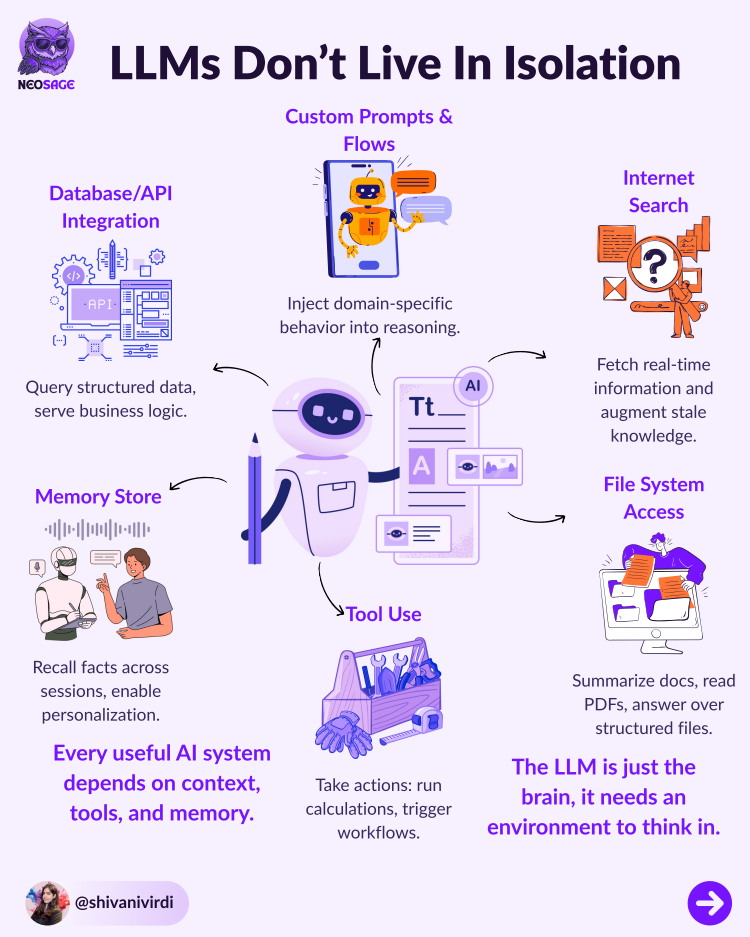
\includegraphics[width=\linewidth,keepaspectratio]{aiagents9}
		\end{center}
    \end{column}
  \end{columns}
   
\end{frame}


%%%%%%%%%%%%%%%%%%%%%%%%%%%%%%%%%%%%%%%%%%%%%%%%%%%%%%%%%%%
\begin{frame}[fragile]\frametitle{The Integration Problem}

\begin{columns}
    \begin{column}[T]{0.5\linewidth}
      \begin{itemize}
        \item Every feature requires custom wrappers
        \item Updates often break existing logic
        \item M apps $\times$ N tools = scaling nightmare
      \end{itemize}

    \end{column}
    \begin{column}[T]{0.5\linewidth}
		\begin{center}
		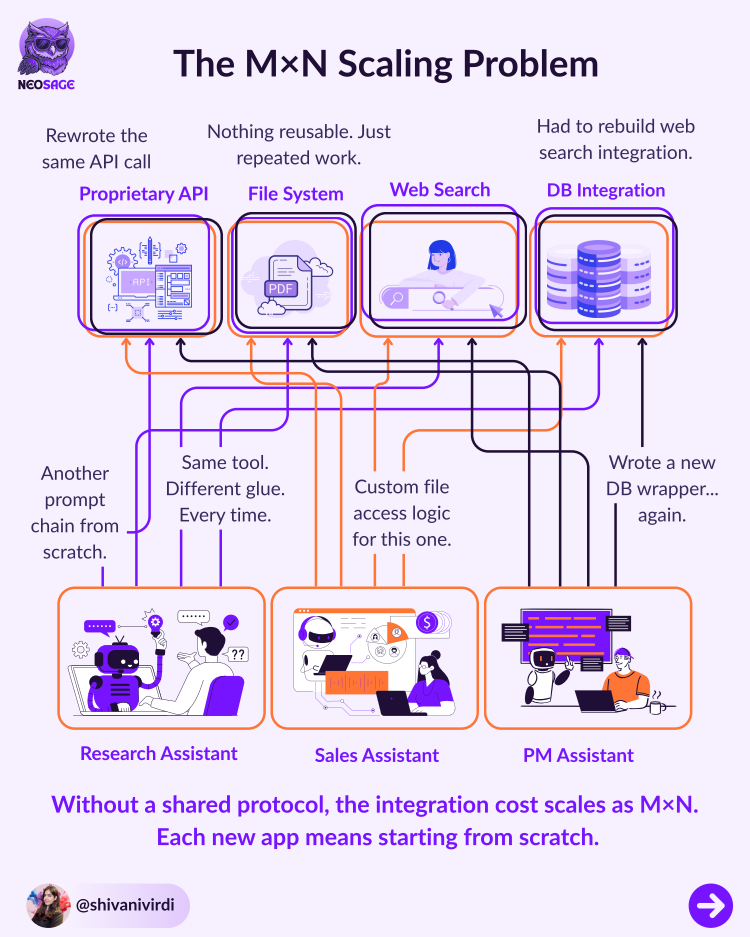
\includegraphics[width=\linewidth,keepaspectratio]{aiagents11}
		\end{center}
    \end{column}
  \end{columns}
  
\end{frame}

%%%%%%%%%%%%%%%%%%%%%%%%%%%%%%%%%%%%%%%%%%%%%%%%%%%%%%%%%%%
\begin{frame}[fragile]\frametitle{Enter MCP: USB-C for AI}
\begin{columns}
    \begin{column}[T]{0.5\linewidth}
      \begin{itemize}
        \item Shared protocol for AI-to-tool connections
        \item One-time tool exposure works with all models
        \item No wrappers, less chaos, easy reuse
      \end{itemize}

    \end{column}
    \begin{column}[T]{0.5\linewidth}
		\begin{center}
		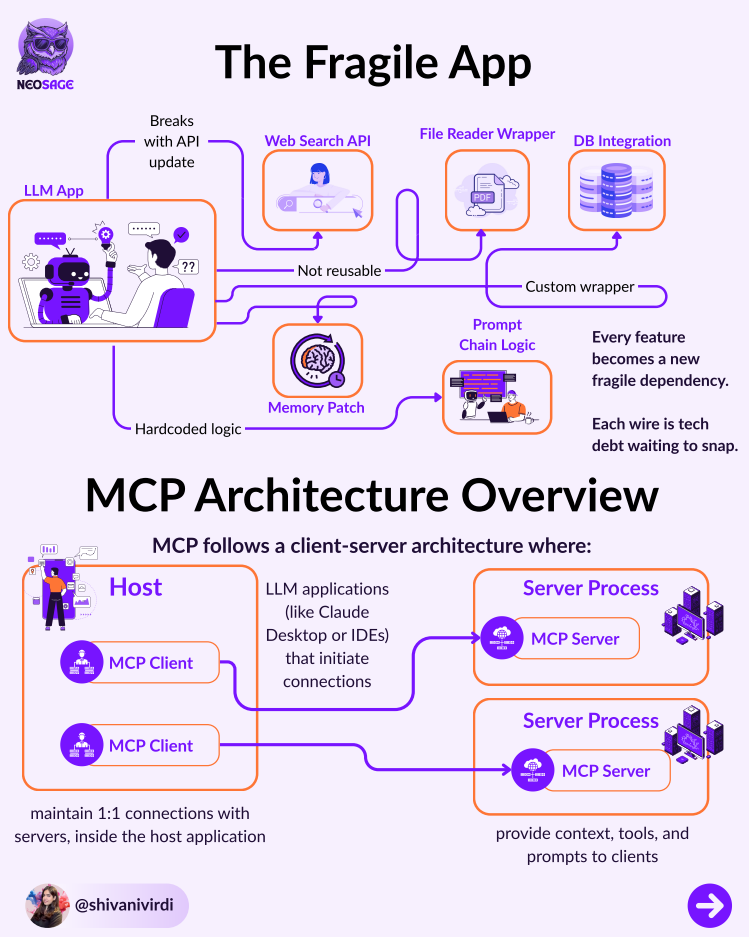
\includegraphics[width=\linewidth,keepaspectratio]{aiagents10}
		\end{center}
    \end{column}
  \end{columns}
\end{frame}


%%%%%%%%%%%%%%%%%%%%%%%%%%%%%%%%%%%%%%%%%%%%%%%%%%%%%%%%%%%
\begin{frame}[fragile]\frametitle{How MCP Works?}
\begin{columns}
    \begin{column}[T]{0.5\linewidth}
      \begin{itemize}
        \item Host: the AI app (e.g., Claude Desktop)
        \item Client: bridge that speaks MCP
        \item Server: where tools, files, prompts live
      \end{itemize}

    \end{column}
    \begin{column}[T]{0.5\linewidth}
		\begin{center}
		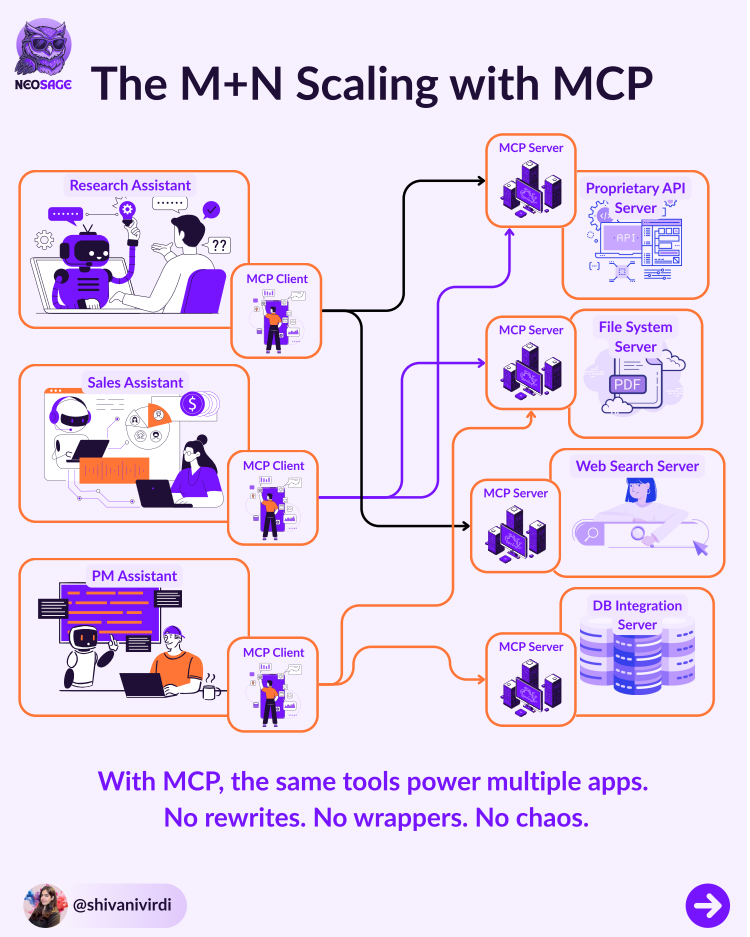
\includegraphics[width=\linewidth,keepaspectratio]{aiagents12}
		\end{center}
    \end{column}
  \end{columns}
\end{frame}

%%%%%%%%%%%%%%%%%%%%%%%%%%%%%%%%%%%%%%%%%%%%%%%%%%%%%%%%%%%
\begin{frame}[fragile]\frametitle{Clean, Typed Communication}
\begin{columns}
    \begin{column}[T]{0.5\linewidth}
      \begin{itemize}
        \item Uses JSON-RPC for structured messaging
        \item Modular design enables reuse
        \item Protocol simplifies complex system behavior
      \end{itemize}

    \end{column}
    \begin{column}[T]{0.5\linewidth}
		\begin{center}
		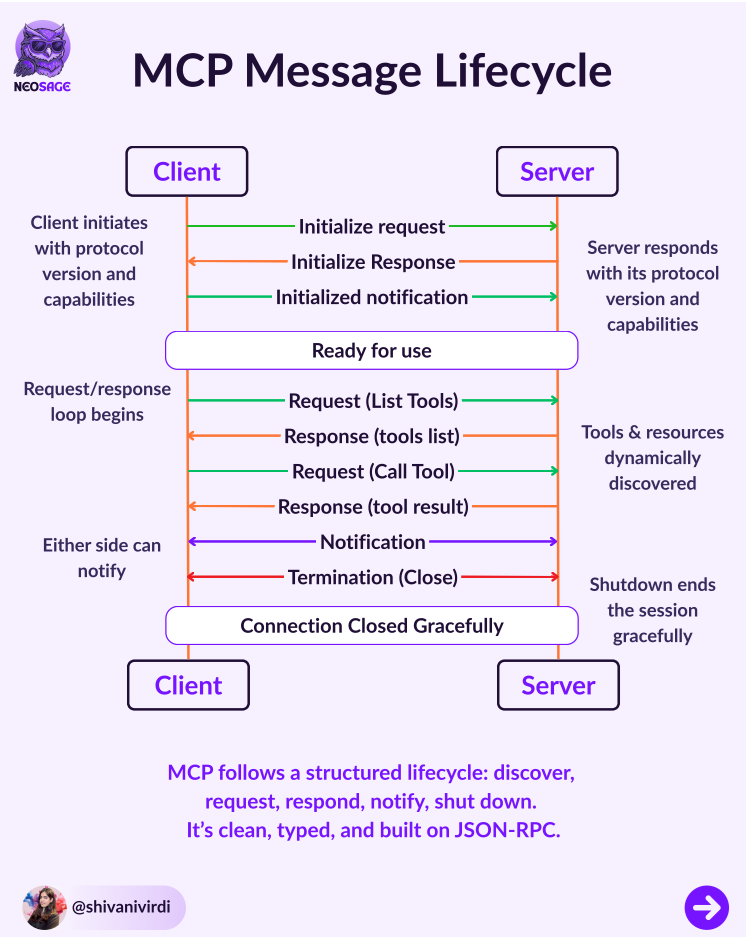
\includegraphics[width=\linewidth,keepaspectratio]{aiagents13}
		\end{center}
    \end{column}
  \end{columns}
\end{frame}

%%%%%%%%%%%%%%%%%%%%%%%%%%%%%%%%%%%%%%%%%%%%%%%%%%%%%%%%%%%
\begin{frame}[fragile]\frametitle{From Demos to Real Systems}


      \begin{itemize}
        \item MCP transforms fragile demos into scalable systems
        \item Reduces engineering overhead
        \item Enables AI software that ships and lasts
      \end{itemize}

	
\end{frame}

%%%%%%%%%%%%%%%%%%%%%%%%%%%%%%%%%%%%%%%%%%%%%%%%%%%%%%%%%%%
\begin{frame}[fragile]\frametitle{From Demos to Real Systems}

\begin{columns}
    \begin{column}[T]{0.5\linewidth}
		\begin{center}
		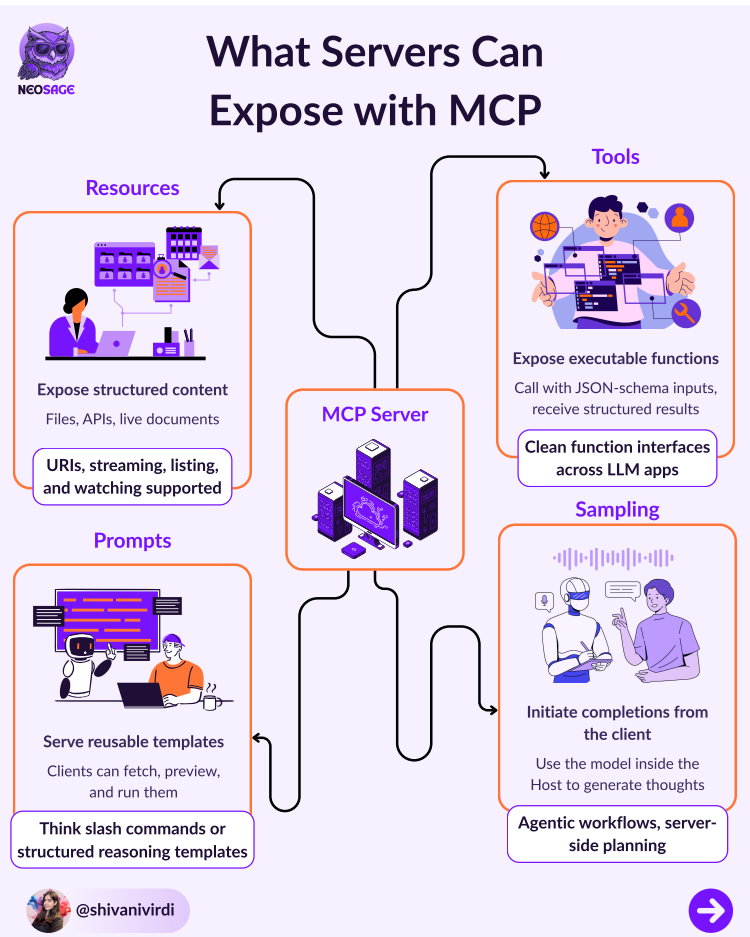
\includegraphics[width=\linewidth,keepaspectratio]{aiagents14}
		\end{center}

    \end{column}
    \begin{column}[T]{0.5\linewidth}
		\begin{center}
		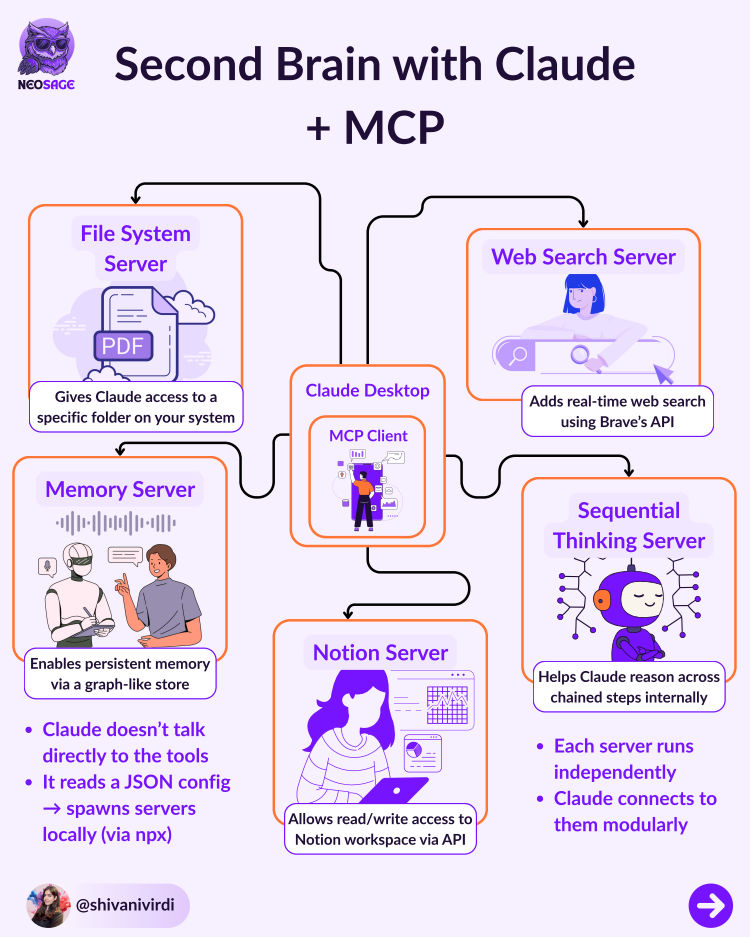
\includegraphics[width=\linewidth,keepaspectratio]{aiagents15}
		\end{center}
    \end{column}
  \end{columns}
  


\end{frame}

%%%%%%%%%%%%%%%%%%%%%%%%%%%%%%%%%%%%%%%%%%%%%%%%%%%%%%%%%%%
\begin{frame}[fragile]\frametitle{Some Opposition to MCP \ldots}
    \begin{itemize}
        \item Fancy acronyms often solve imaginary problems
        \item Overengineered MCP layers complicate agent-API flow
        \item Hype drives architecture-not actual needs
        \item Direct API calls are faster and clearer
        \item Lower latency and reduced system complexity
        \item Easier to debug, scale, and maintain	
		\item Skip the MCP if your API already works
        \item Avoid unnecessary layers for trend's sake
        \item Prioritize shipping over architecture theater
    \end{itemize}
\end{frame}


%%%%%%%%%%%%%%%%%%%%%%%%%%%%%%%%%%%%%%%%%%%%%%%%%%%%%%%%%%%%%%%%%%%%%%%%%%%%%%%%%%
\begin{frame}[fragile]\frametitle{}
\begin{center}
{\Large Zerodha Kite MCP Server}
\end{center}
\end{frame}
